\documentclass[conference]{IEEEtran}
\usepackage{enumitem}
\usepackage{amsmath}
\usepackage{amssymb}
\usepackage{listings} 
\usepackage{graphicx}
\usepackage{url}
\usepackage{tabularx}
\usepackage{subfigure}
\usepackage{lipsum}
\usepackage{multirow}

%\newtheorem*{definition}{Definition}

\begin{document}
%	\title{CSE 802 Pattern Recognition \& Analysis  \\
%		Spring 2017, Project Final Report}
	\title{Unconstrained Human Face Recognition: Challenge}

%	\author{Deliang Yang\hspace{1in}Mengying Sun\\A50836814\hspace{1.3 in}A49087906}
	\author{\IEEEauthorblockN{Deliang Yang}
		\IEEEauthorblockA{Depoartment of Electrical and\\Computer Engineering\\
			A50836814\\
			yangdeli@msu.edu}
		\and
		\IEEEauthorblockN{Mengying Sun}
		\IEEEauthorblockA{Depoartment of Computer \\ Science and Engineering \\A49087906
			\\sunmeng2@msu.edu}}
	\maketitle


\begin{abstract}

In this project, we propose a deep network model to perform unconstrained face recognition task. The performance of the model has been evaluated and compared with traditional methods.

\end{abstract}

\section{Introduction}

Face detection and recognition has been both attracting and challenging in modern society. It becomes possible through a wide variety of images available online and large database system, also achieves higher detection rate via rapidly developed techniques such as deep neural networks. However, it remains challenging due to large feature size and complex noise. More efforts are still to be devoted in pattern recognition community by improving algorithms and method for successful face detection. 

In this paper, we propose a deep convolutional network frame to improve detection rate based on CASIA and LFW database \cite{LFWTech}. Results demonstrate that the proposed network significantly improves human face recognition rate compared to other traditional methods. Verification rates of over 48\% at false accept rate (FAR) of 0.1\% are achieved by both PCA and LDA method.

\section{Project Methods and Design}

\subsection{Workflow}

The basic workflow is described as follows. First we train the deep network model with CASIA Webface Database \cite{casia}. The model includes a fully connected layer at the end of the network to classify the input images to one of the 10,575 classes. Then we feed the network with LFW database images, and use the model intermediate hidden layer output as features. Those features will be extract once again by PCA or LDA. Finally, the features from LFW will be evaluated via 10 trails cross validation in BLUFR protocol \cite{yi2014learning}. 

\subsection{Deep Network Model Structure}

There are 8 convolutional neural network (CNN) \cite{lawrence1997face} layers in our model. The sequential structure and corresponding unit sizes are shown in Table \ref{mdl_stru}. These 8 CNN layers will be grouped into 4 larger layers. At the end of each large layers, ReLU (Rectifier Linear Unit) will be applied as activation function. To reduce the feature dimension, pooling layers are employed. The first three activation functions will be followed by MaxPooling layers with kernel size 2x2. The final pooling layer is AveragePooling, with kernel 6x6. After the average pooling, the feature dimension is 1x1 for each unit. The final pooling output is flattened and fed into a dropout layer to set random values with a proportion of 60\% to 0, which prevents model from overfitting. The fully connected layers and Softmax activation will extract the output label of the input sample.

Compared to the baseline model provided in project guideline, the changes we made are as follows: 1) remove two convolutional layers because we encounter ``not enough dimension error'' when compiling the model; 2) slightly change the number of the filter size of each CNN layer.

\setlength\extrarowheight{3pt}
\begin{table}[]
	\centering
	\caption{Deep network structure in the project}
	\label{mdl_stru}
	\begin{tabular}{|l|r|r|}
		\hline
		Layer                 & Output dim                   & Parameters \# \\ \hline
		conv2d\_1             & 110 $\times$ 110 $\times$ 32 & 896           \\ \hline
		conv2d\_2             & 108 $\times$ 108 $\times$ 64 & 18496         \\ \hline
		activation\_1 ReLU    &                              &               \\ \hline
		max\_pooling2d\_1     & 54 $\times$ 54 $\times$ 64   &               \\ \hline
		conv2d\_3             & 52 $\times$ 52 $\times$ 64   & 36928         \\ \hline
		conv2d\_4             & 50 $\times$ 50 $\times$ 128  & 73856         \\ \hline
		activation\_2 ReLU    &                              &               \\ \hline
		max\_pooling2d\_2     & 25 $\times$ 25 $\times$ 128  &               \\ \hline
		conv2d\_5             & 23 $\times$ 23 $\times$ 128  & 147584        \\ \hline
		conv2d\_6             & 21 $\times$ 21 $\times$ 256  & 295168        \\ \hline
		activation\_3 ReLU    &                              &               \\ \hline
		max\_pooling2d\_3     & 10 $\times$ 10 $\times$ 256  &               \\ \hline
		conv2d\_7             & 8 $\times$ 8 $\times$ 256    & 590080        \\ \hline
		conv2d\_8             & 6 $\times$ 6 $\times$ 512    & 1180160       \\ \hline
		activation\_4 ReLU    &                              &               \\ \hline
		average\_pooling2d\_1 & 1 $\times$ 1 $\times$ 512    &               \\ \hline
		flatten\_1            & 512                          &               \\ \hline
		dropout\_1 (60\%)     & 512                          &               \\ \hline
		dense\_1              & 10575                        & 5424975       \\ \hline
		activation\_5 Softmax &                              &               \\ \hline
	\end{tabular}
\end{table}

\setlength\extrarowheight{3pt}
\begin{table*}[!ht]
	\centering
	\caption{Comparison of the BLUFR evaluation results of the deep network and traditional methods}
	\label{eval_result}
	\begin{tabular}{|l|r|r|r|r|r|r|}
		\hline
		& \multicolumn{2}{r|}{LE (Learning-based descriptors)} & \multicolumn{2}{r|}{High Dimensional LBP} & \multicolumn{2}{r|}{CNN Model} \\ \hline
		Feature size                       & \multicolumn{2}{r|}{20736}                           & \multicolumn{2}{r|}{127440}               & \multicolumn{2}{r|}{512}        \\ \hline
		Method                             & PCA                      & LDA                       & PCA                 & LDA                 & PCA             & LDA            \\ \hline
		Verification @ FAR = 0.1\%:        & 8.94\%                   & 20.95\%                   & 8.20\%              & 30.86\%             & 48.38\%         & 48.46\%        \\ \hline
		Open-set Identification @ Rank = 1 & 4.93\%                   & 13.39\%                   & 5.32\%              & 17.46\%             & 4.37\%          & 5.18\%         \\ \hline
	\end{tabular}
\end{table*}

\subsection{Software Framework}

The library we use to build the deep network is \texttt{Keras} \cite{chollet2015keras}, which employs the Google open source deep network library, \texttt{Tensorflow} \cite{abadi2016tensorflow} as backend. 

In data preprocessing, the keras built-in class \texttt{ImageDataGenerator} is used to randomly selecting samples from the CASIA database, which will prevent the model from overfitting within a small set of recently trained classes. The image preprocessing class also support random rotation, horizontal shift, vertical shift, horizontal flip and so on, which actually generates larger number of training samples than the original database. It is believed this method will eventually improve the robustness and accuracy while applied to unconstrained face recognition task.

\begin{figure}
	\centering 
	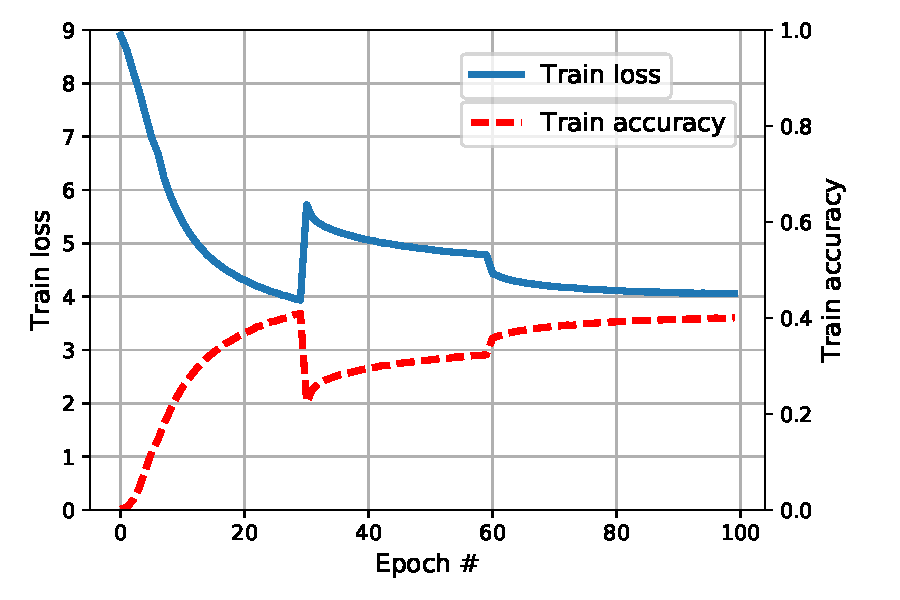
\includegraphics[width=7.2cm]{./train_loss_acc_log.pdf}
	\caption{Train loss and accuracy vs. number of epochs}
	\label{train_loss_acc} %% label for entire figure 
\end{figure}

\subsection{Hyper Parameters}

In our project we use the following hyper parameters settings:

\begin{itemize}
	\item Optimizer: AdaDelta \cite{zeiler2012adadelta}
	\item Learning rate: 1.0
	\item Parameter update decaying control factor $\rho$: 0.95
	\item Fuzzy factor $\varepsilon$: 1e-8
	\item Batch size: 128
	\item Epoch: 100
	\item Loss: categorical cross entropy
	\item Random rotation degree limit: 20
	\item Random horizontal shift limit: 0.2
	\item Random vertical shift limit: 0.2
\end{itemize}
\begin{figure}
	\centering 
	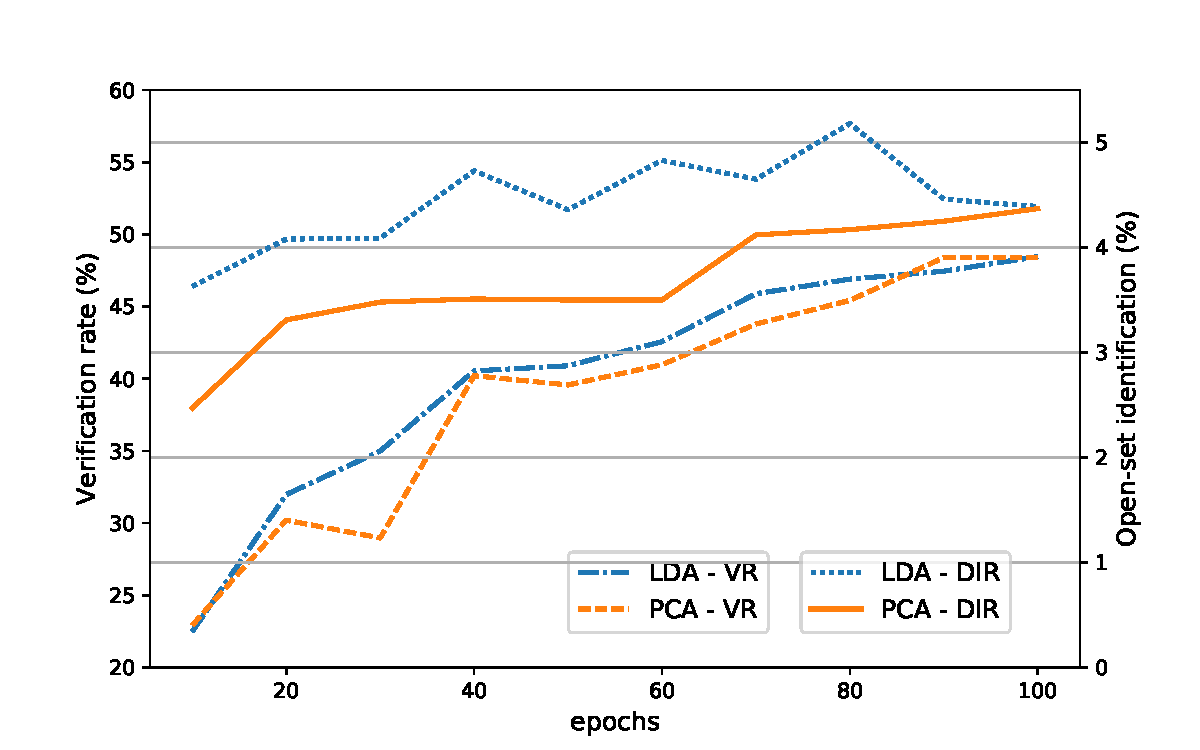
\includegraphics[width=7.7cm]{./cnn_model7_vr_dir.pdf}
	\caption{Train loss and accuracy vs. number of epochs}
	\label{cnn_vr_dir} %% label for entire figure 
\end{figure}

\section{Evaluation and Result}

The training process will be evaluated by training loss and accuracy. The test performance will be benchmarked by verification rate at FAR = 0.1\% (VR) and open-set identification at Rank = 1 (DIR) in BLUFR protocol.

\subsection{Training Performance}

The model training loss and accuracy curve can be seen in Fig. \ref{train_loss_acc}. The first 30 epochs are trained without real time data augmentation during preprocessing. As we can see, with augmentation, training process slows down, and the loss increases, accuracy decreases. Because the model hasn't fit the augmented pictures before. Although the train accuracy is lower than 40\% in the CASIA dataset, the actually verification rate in LFW can reach up to 48\% at FAR 0.1\% for both PCA and LDA feature extraction methods, which will be demonstrated in the following section. 

The trend of VR and DIR varying with the training epochs is shown in Fig. \ref{cnn_vr_dir}. As we can notice, after introducing data augmentation at preprocessing, the VR increases about 10\% for both PCA and LDA method from 30th epoch to 40th one. There is some boost in DIR under LDA method, however DIR under PCA remains almost the same. 

\subsection{LFW Dataset Evaluation}

Evaluations are taken on three different types of features via two approaches: i) Learning-based descriptors; ii) High dimensional LBP; iii) CNN extracted features each is evaluated through both PCA and LDA. High dimensional LBP has the largest feature size, which is 127,440, while CNN extracted features has least dimension, which is 512. The results can be found at Table \ref{eval_result}. 

\begin{figure*}
	\centering 
	\subfigure[~Verification ROC curve with PCA feature extraction]{
		\label{vr_pca} % label for first subfigure
		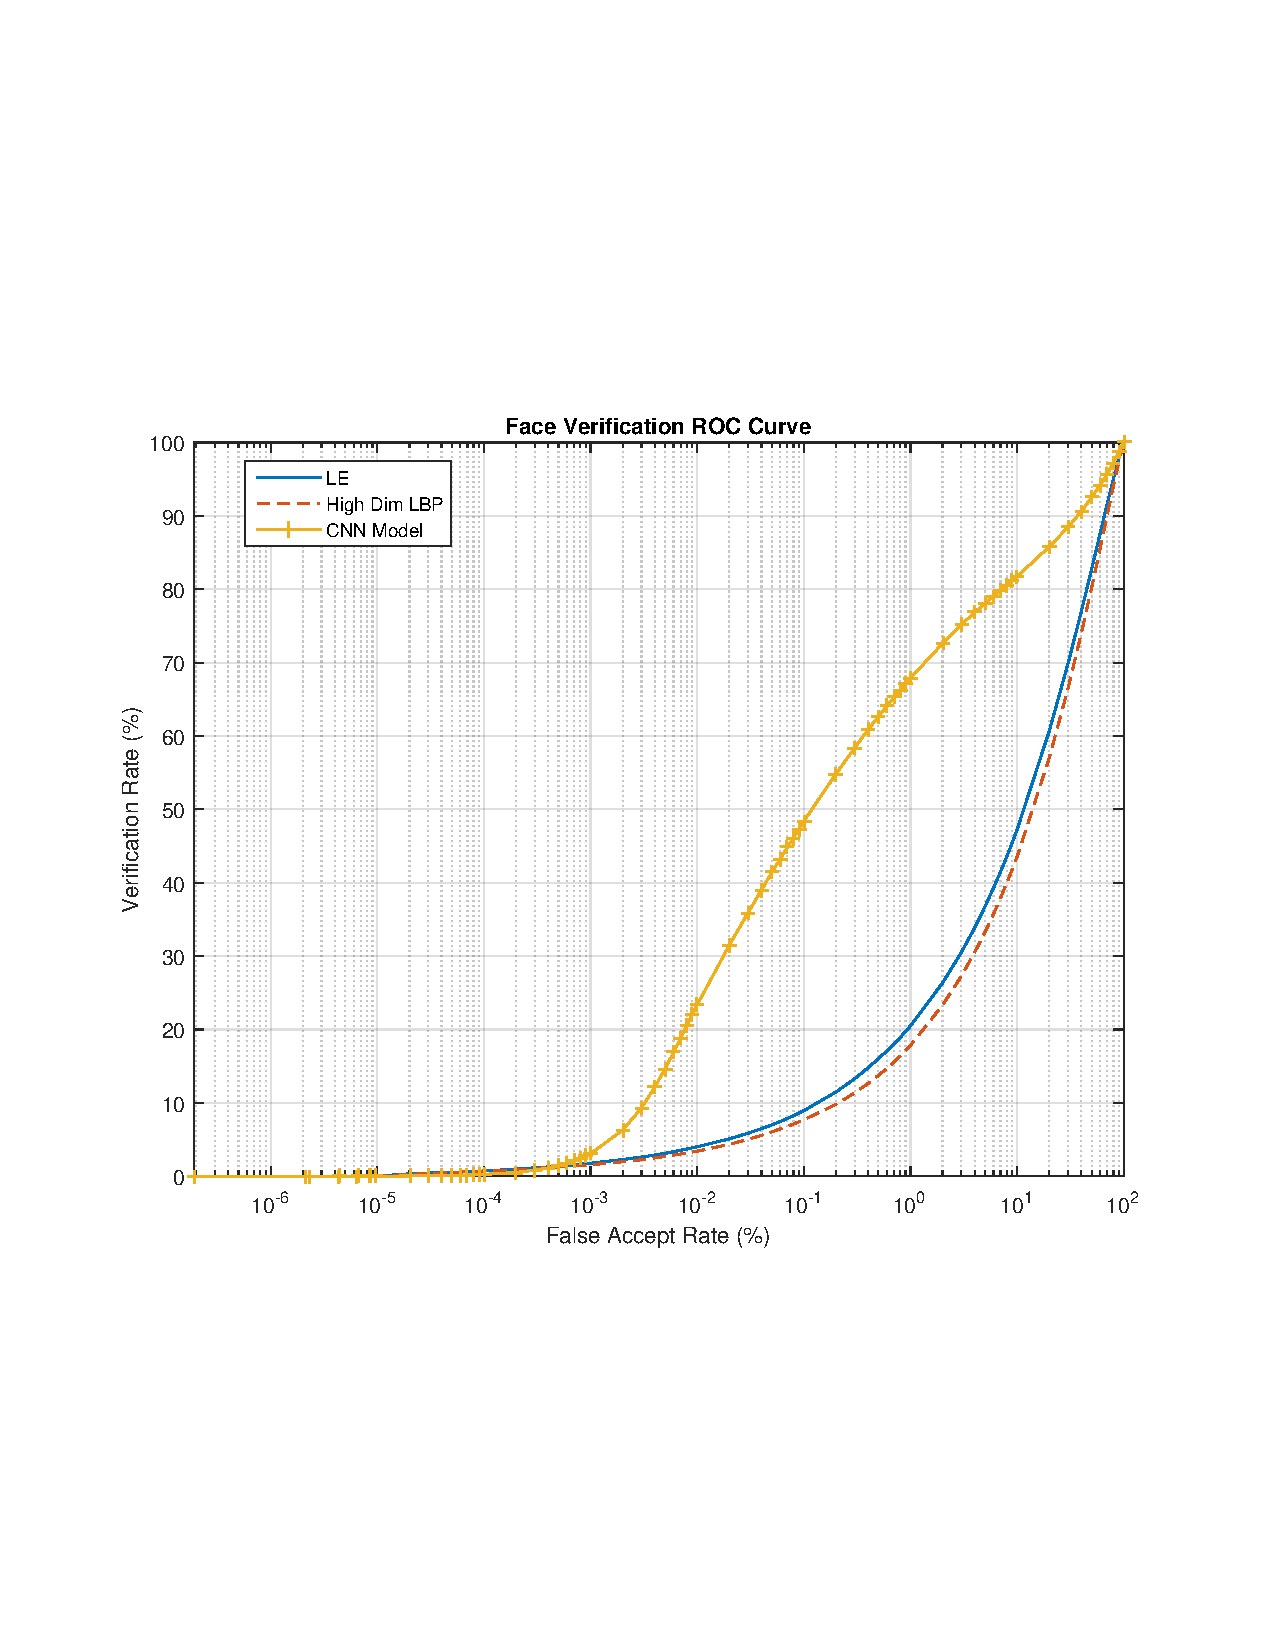
\includegraphics[width=6.7cm, trim={1.2cm 6.4cm 1.2cm 6.1cm}]{./all_pca_verificationROC.pdf}}
	\hspace{0.25in} 
	\subfigure[~Open-set identification ROC curve at Rank 1 with PCA feature extraction]{
		\label{dir_pca} % label for second subfigure 
		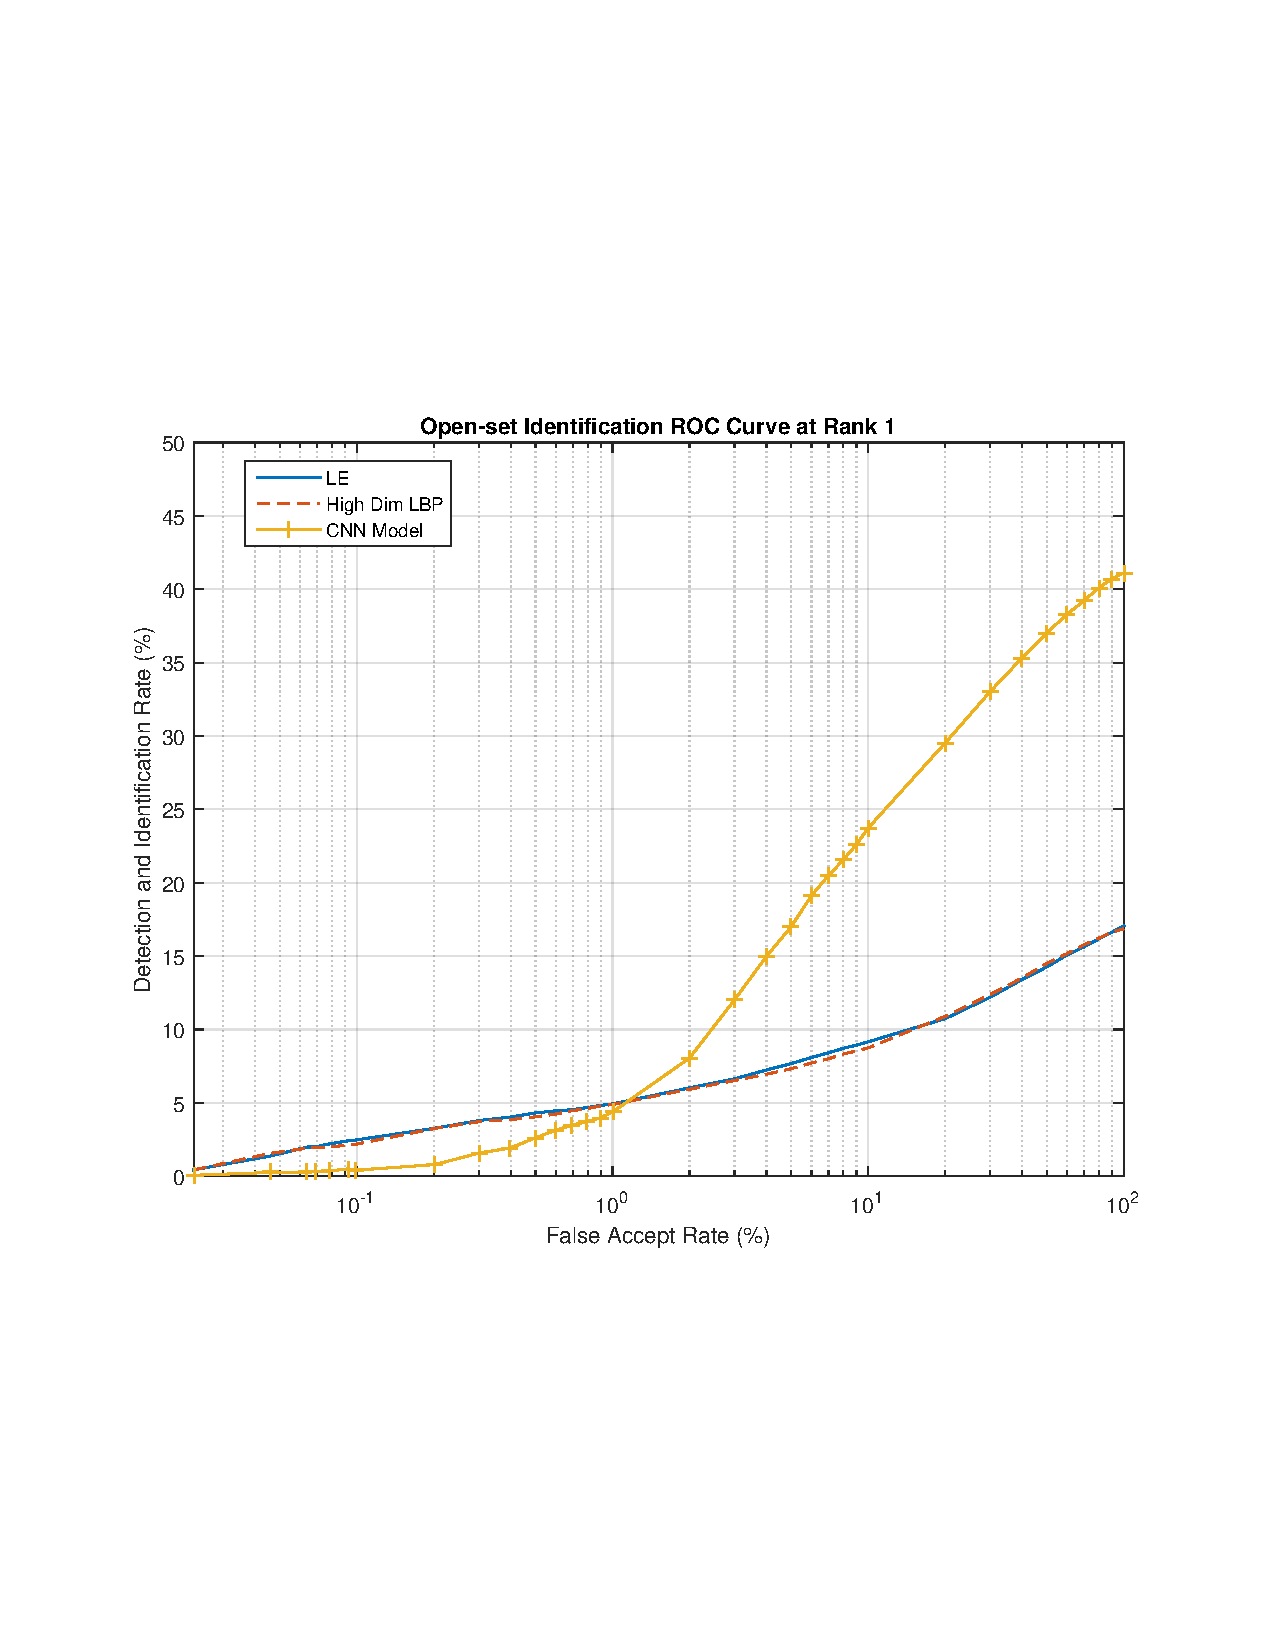
\includegraphics[width=6.7cm, trim={1.2cm 6.4cm 1.2cm 6.1cm}]{./all_pca_rank1.pdf}}
	%	   \hspace{0.05in} 
	\subfigure[~Verification ROC curve with LDA feature extraction]{
		\label{vr_lda} % label for second subfigure 
		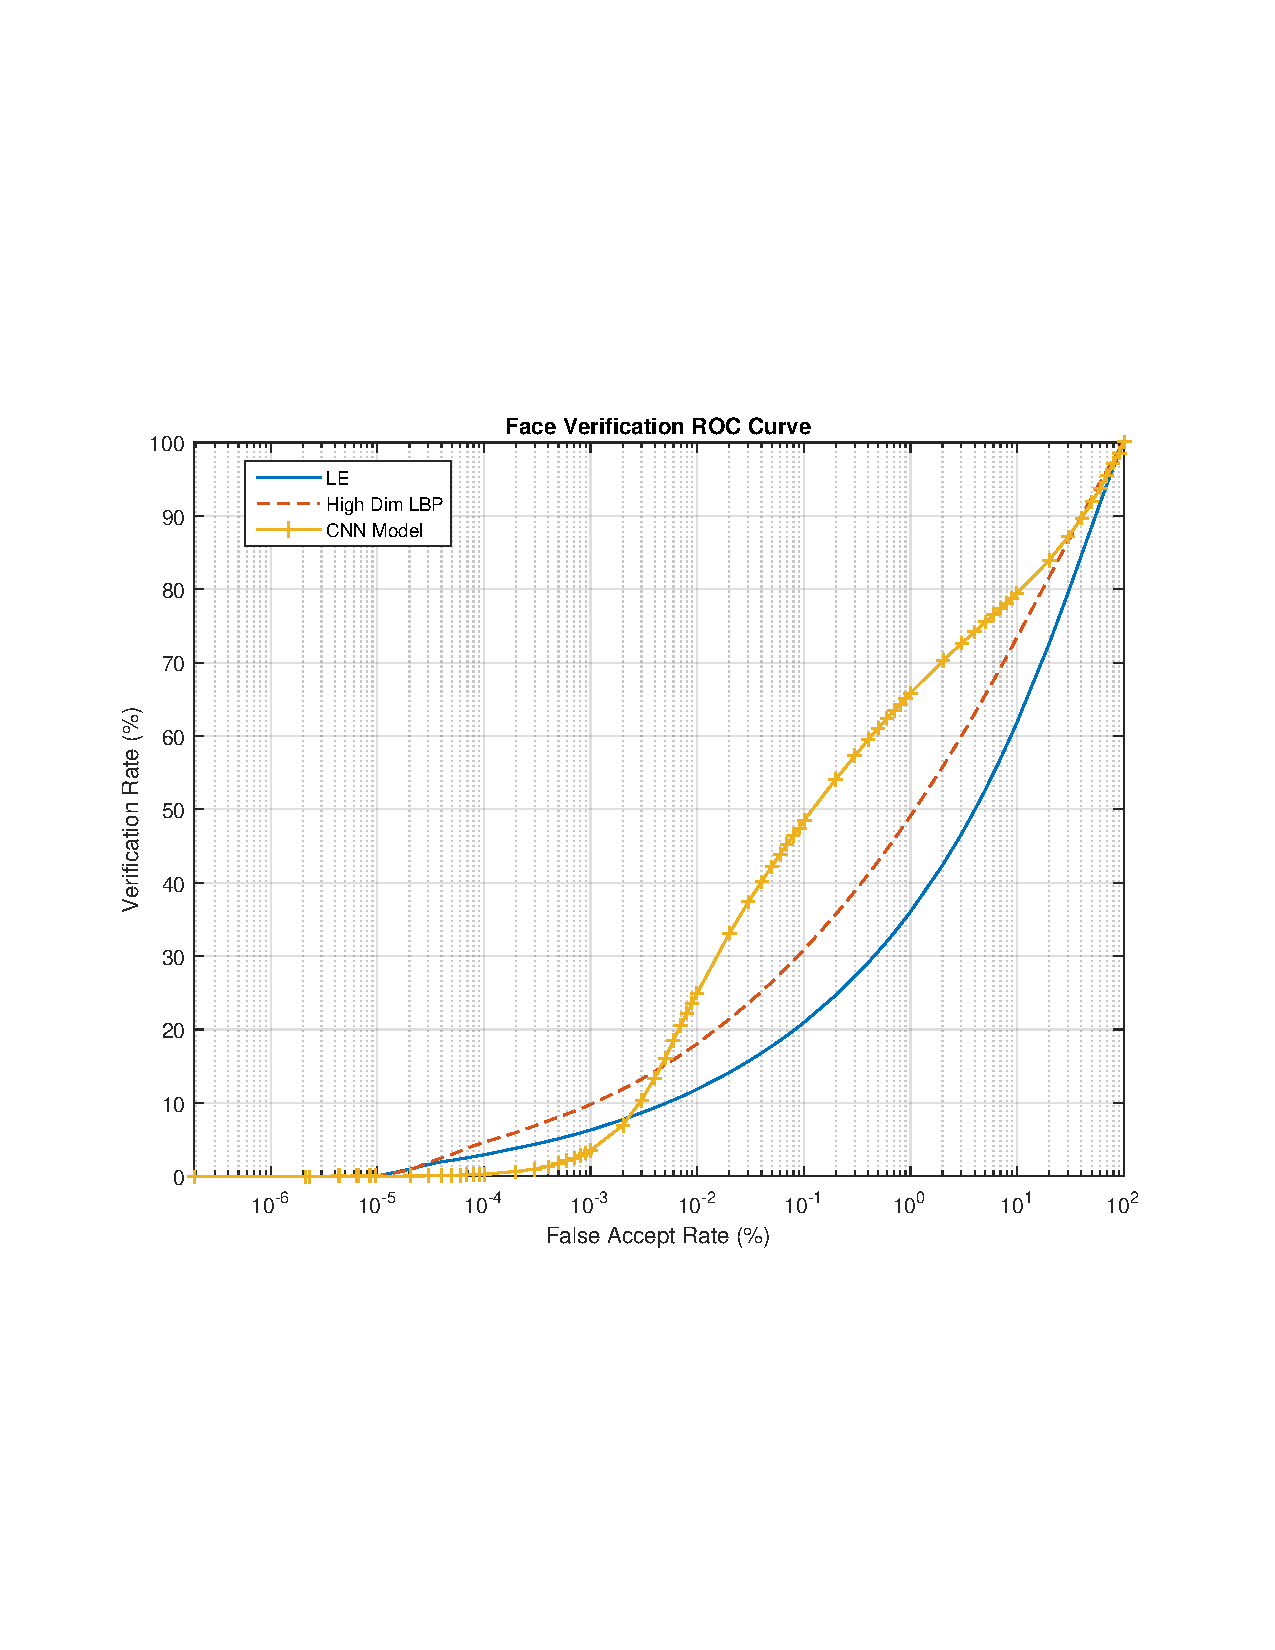
\includegraphics[width=6.7cm, trim={1.2cm 6.4cm 1.2cm 6.1cm}]{./all_lda_verificationROC.pdf}}
	\hspace{0.25in} 
	\subfigure[~Open-set identification ROC curve at Rank 1 with LDA feature extraction]{
		\label{dir_lda} % label for second subfigure 
		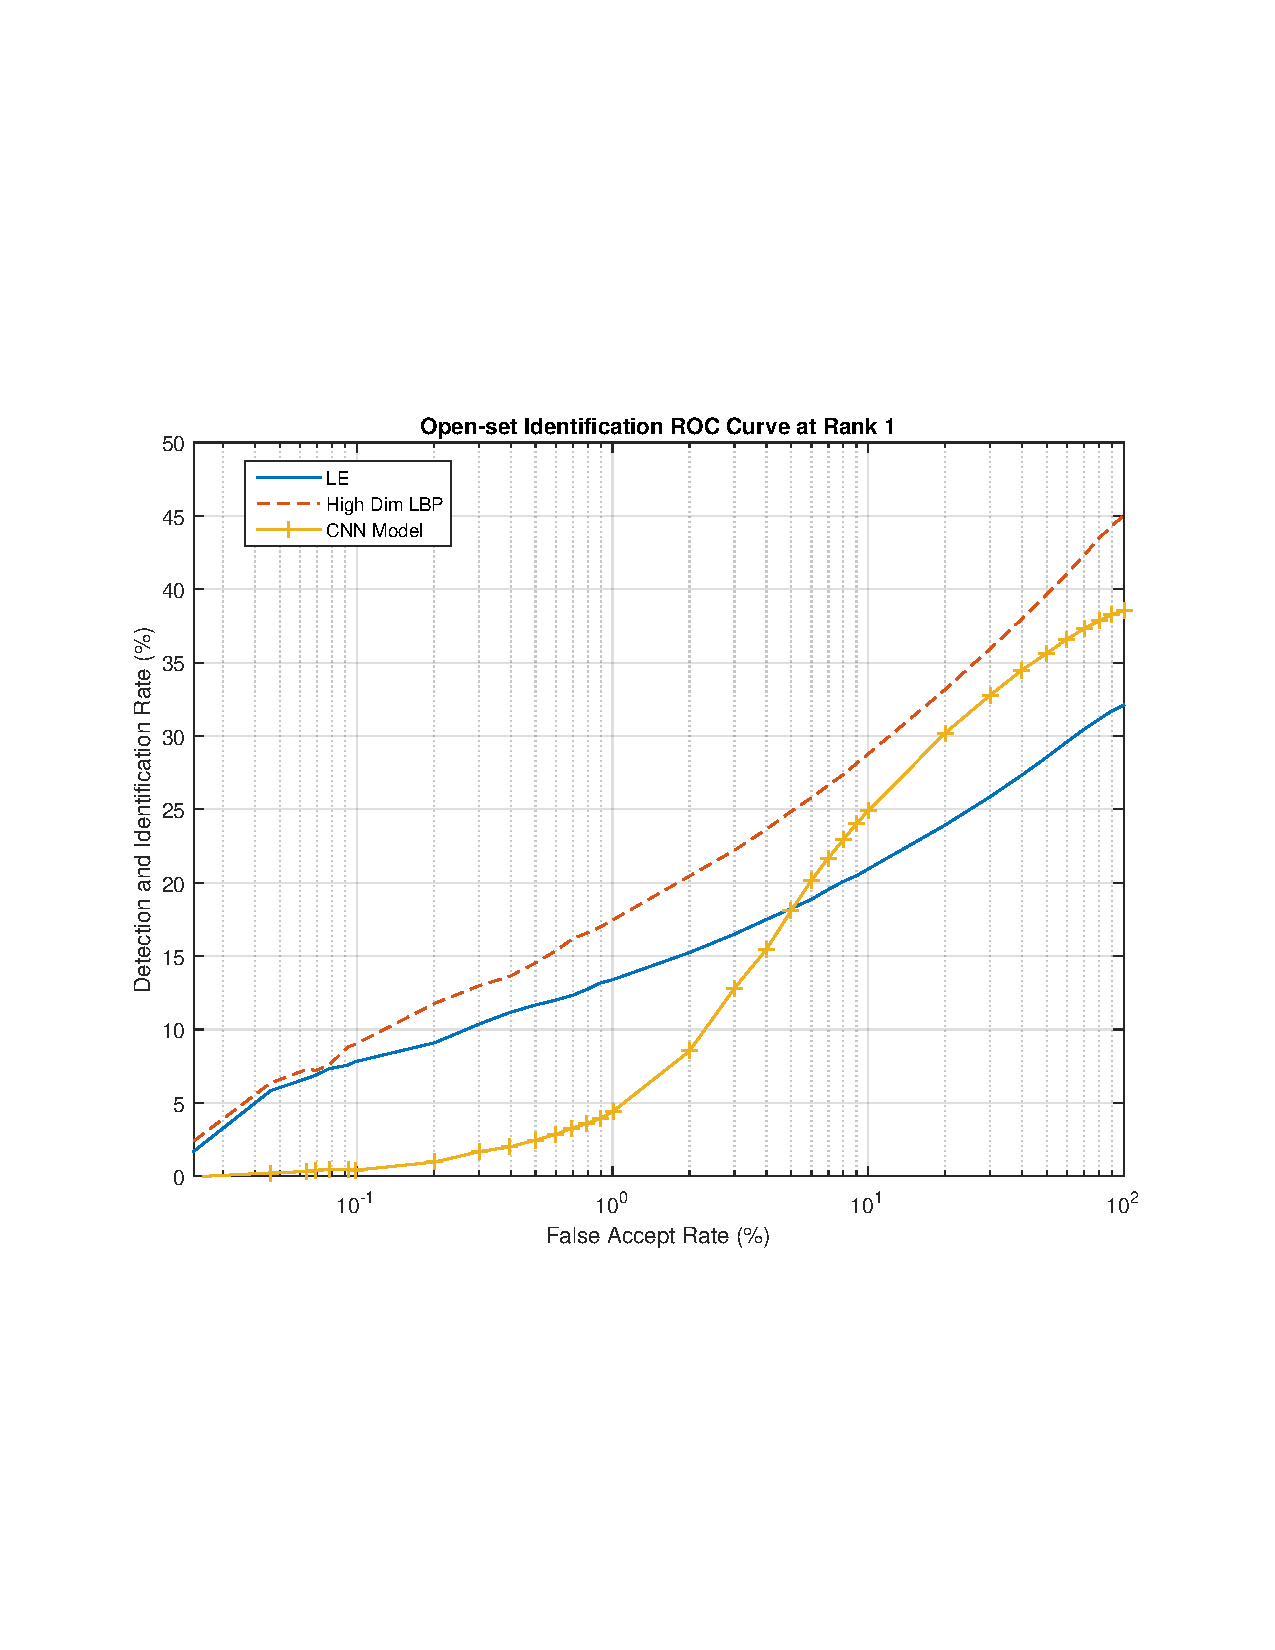
\includegraphics[width=6.7cm, trim={1.2cm 6.4cm 1.2cm 6.1cm}]{./all_lda_rank1.pdf}}
	\caption{ROC curve of different features and corresponding feature extraction methods.}
	\label{test_result} %% label for entire figure 
\end{figure*}

LDA outperforms PCA for all three features in the same feature setting, with high dimensional LBP serves the best prediction accuracy for open-set identification among all features, where 17.46\% is achieved under LDA method. A highest verification rate of 48.46\% is achieved by CNN extracted feature under LDA method. Feature extracted by our proposed CNN achieves open-set identification rate of only 4.37\% and 5.18\% at Rank 1 for PCA and LDA method respectively. 

Figure \ref{test_result} shows the ROC curve at different false accept rate for each feature under different methods. In verification with PCA, CNN model has highest values across all the FAR. In LDA method, LE and LBP perform better than CNN model at low FAR, which means CNN model may failed in restrict condition. For open-set identification in PCA method, CNN model also has lower value than LE and high dimensional LBP in low FAR range, but it increases dramatically as FAR increases. However in LDA method, the extracted feature from LBP has higher discriminative ability than CNN model across most of the FAR values. This indicate that discriminability of features extracted from CNN may not be augmented by LDA methods. 

\section{Teamwork}

Teamwork is appreciated along with the completion of the project. Basically the job is divided as follows:

\begin{itemize}
	\item Mengying finishes the BLUFR protocol framework processing functions and run the PCA and LDA results on LE (learning-based descriptors) and high dimensional LBP (local binary patterns) feature extractor. 
	
	\item Deliang builds the framework of deep network with Keras with tensorflow backend. He also writes the code that converts the raw LFW images to feature matrix. 
\end{itemize}


Both of the two team members work together to run the code on HPCC successfully. We also collaborate to tune parameters and update the network layers.

Progress report, presentation and final report are also finished by teamwork.


\section{Conclusion}

In this project, we use CASIA database to train a deep network model that can extract features for unconstrained face recognition system. The CNN model achieves over 40\% verification rate and 4.73\% open-set identification rate under LDA method in BLUFR protocol and outperforms traditional method such as LE and LBP in many aspects. It is a promising model that can be applied to face recognition. We also want to point out that there are lot of technical tricks that can be done to further improve the performance. 


\bibliographystyle{IEEEtran}
\bibliography{cse802_final_report_ref}  

\end{document}